\testCom
{%Номер задачи
	3.153
}
{%Условие
	условие
}
{%Дано
	дано
}
{%Найти
	найти
}
{%Решение
	%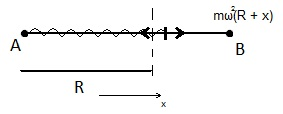
\includegraphics[height=30mm]{3_33.jpg}\\
	Закон Ома для переменного тока:\\
	\[I_m e^{\cancel{i \omega t} + \alpha} \left(R - \frac{i}{\omega C}\right) = U_m \cancel{e^{i \omega t}}\]
	$\alpha = \arctg \omega R C, \quad I_m = \frac{U_m \omega C}{\sqrt{1 + (\omega C R)^2}}$\\
	
}

